\documentclass[12pt]{article}
\usepackage[a4paper,height=23cm]{geometry}
\usepackage[tableposition=top]{caption}
\captionsetup{font=small,labelfont=bf,labelsep=period,singlelinecheck=false,
  width=13cm}
\usepackage{color}
\usepackage{graphicx}
\usepackage{parskip}
\usepackage[hidelinks,linktoc=all,pdfpagemode=None]{hyperref}
\definecolor{darkblue}{rgb}{0.0,0.2,0.6}
\definecolor{darkgray}{rgb}{0.2,0.2,0.2}
\newcommand\blue[1]{\textcolor{darkblue}{#1}}
\newcommand\gray[1]{\textcolor{darkgray}{#1}}
\newcommand\I[1]{\rule{0pt}{#1}}
\newcommand\gt{\raisebox{0.1ex}\textgreater}
\frenchspacing
\setlength\hyphenpenalty{1000}
\hyphenation{calculated mentioning support analyses deriving commonly
  repository}
\begin{document}

\thispagestyle{empty}

\begin{center}
  ~\\[0ex]
  \Large\bfseries SOFIA Transparent\\
  Analytical Framework\\[1.5ex]
  \large{\rm Design and development progress}\\[2.6cm]
  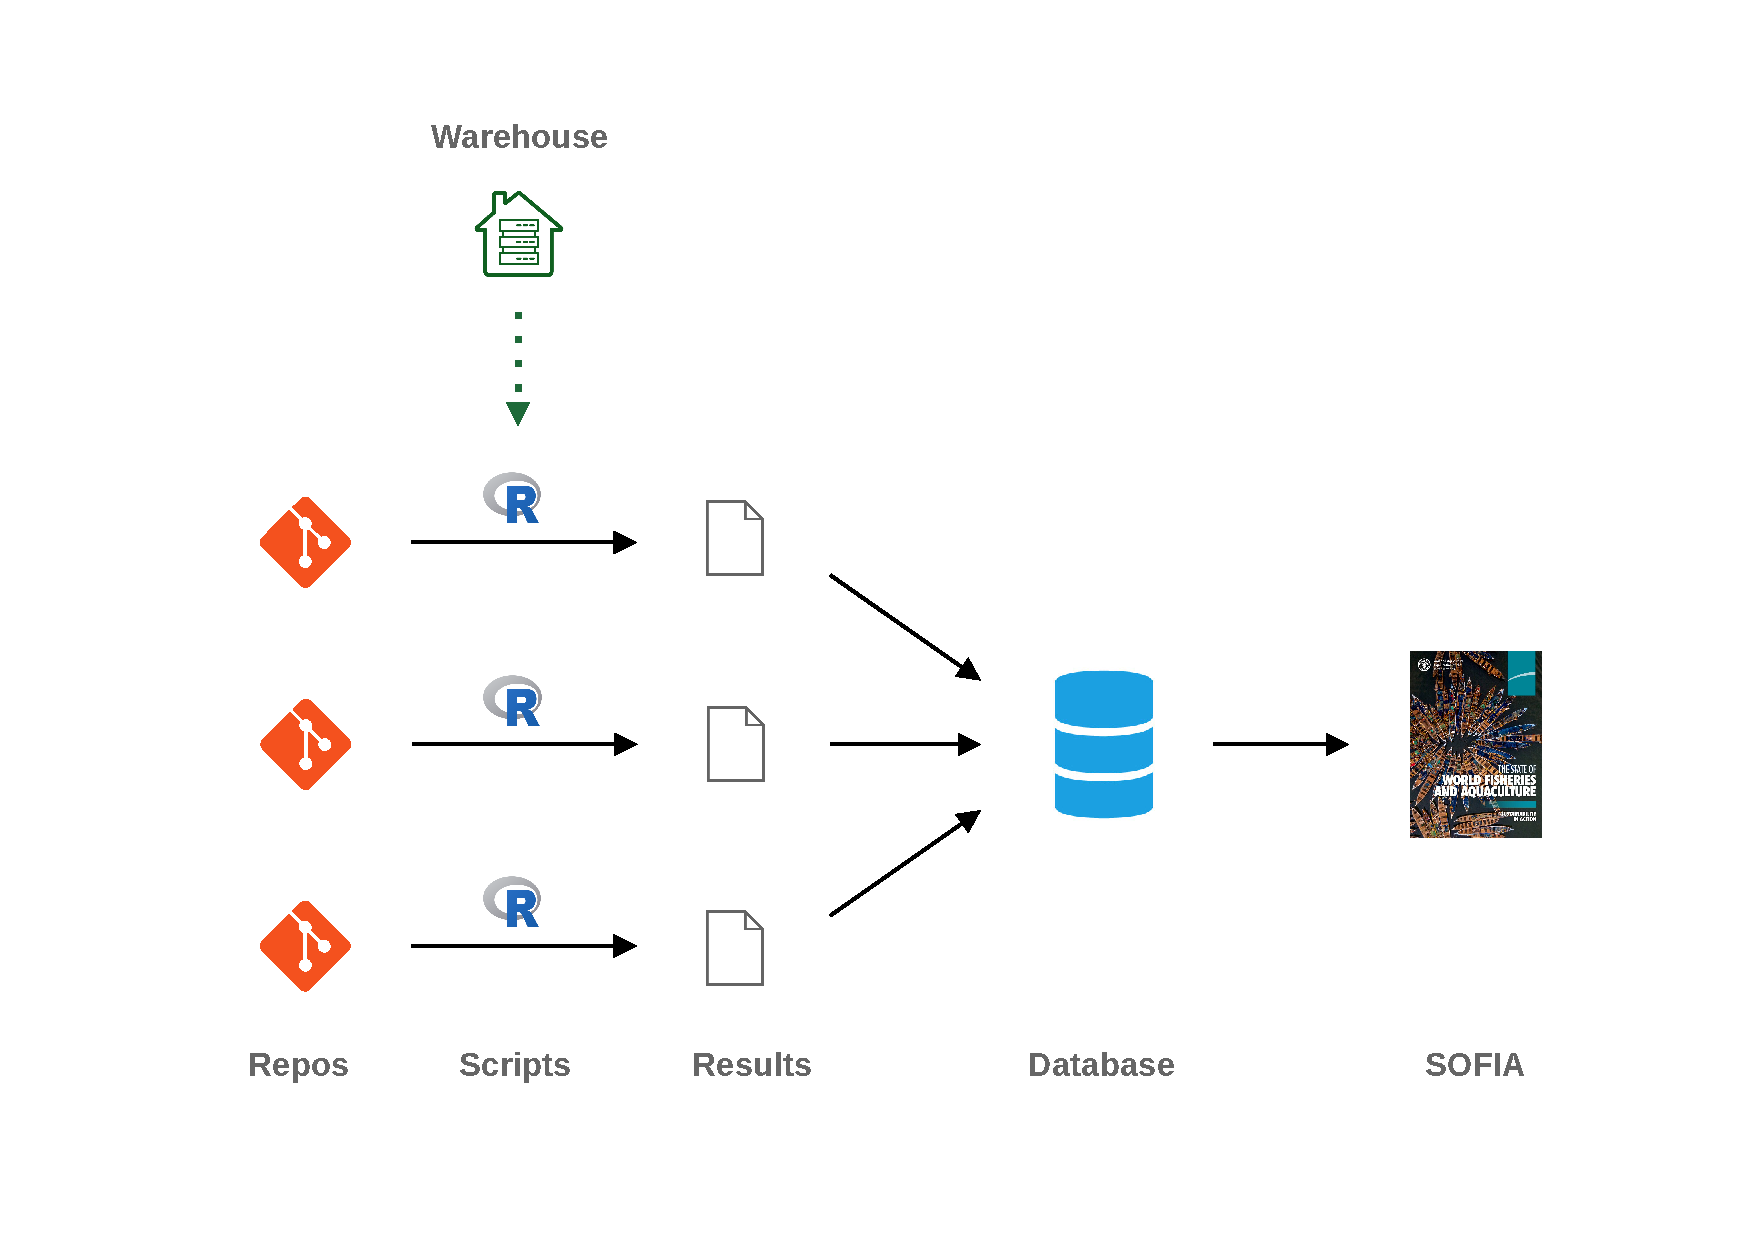
\includegraphics[width=0.64\textwidth]{tsaf_diagram}\\[1.5cm]
  \hspace{-1.5ex}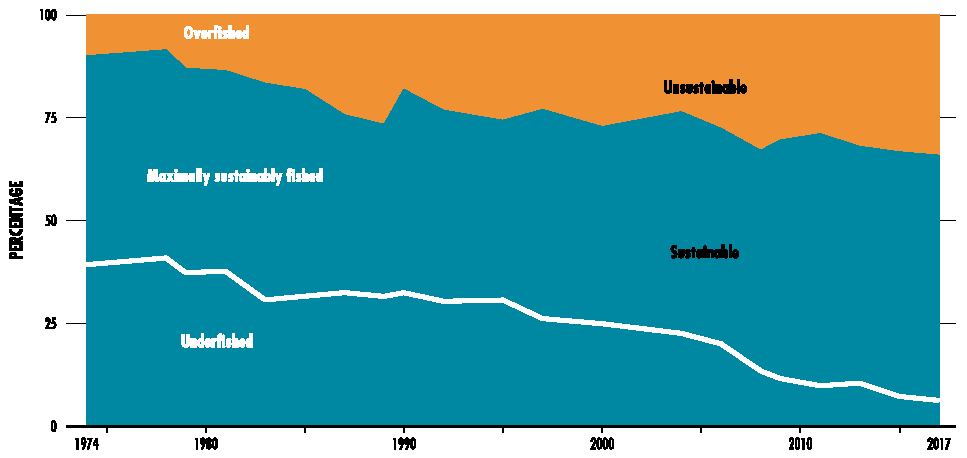
\includegraphics[width=0.75\textwidth]{sofia_fig19}\\[1.8cm]
  \mdseries Arni Magnusson\\[1.6ex]
  December 2021
\end{center}

\newpage

~\vspace{1em}
\setcounter{tocdepth}{2}
\tableofcontents

\newpage

\section{Executive summary}

This report gives a brief overview of the design and development progress of the
new Transparent SOFIA Analytical Framework (TSAF) that was initiated in March
2021. As of December 2021, the design is nearly complete and the implementation
is underway. The overall framework consists of four components:\\[-3ex]

\begin{itemize}
  \item TSAF repositories, where each repository contains one analysis,
  calculating the status of stocks in a given area.\\[-3.5ex]
  \item Input data warehouse, with fisheries data for all areas and
  stocks.\\[-3.5ex]
  \item R package, a collection of utilities that are commonly used in TSAF
  analyses.\\[-3.5ex]
  \item Database, storing the results from all TSAF analyses.\\[-3ex]
\end{itemize}

At the end of this report is an appendix, listing Arni Magnusson's contributions
in 2021 to TSAF design and development.

% ______________________________________________________________________________

\section{Introduction}

\subsection{Background}

In March 2021, Rishi Sharma contacted Arni Magnusson to explore the possibility
of collaboration to design a new way to organize the analysis of the State of
the World Fisheries and Aquaculture (SOFIA). From his years at ICES, Arni had
experience in designing the Transparent Assessment Framework (TAF, ICES 2021)
which is used to organize the stock assessment and advisory workflow for a large
number of ICES stock assessments each year.

The first exploratory step was to convert an existing SOFIA analysis, from a
single monolithic R Markdown document to TAF format, using Area 37 as a
prototype. This was done by creating a GitHub repository and splitting the
analysis into four R scripts: \verb|data.R|, \verb|model.R|, \verb|output.R|,
and \verb|report.R|. Splitting the analysis in this way into discrete steps made
it more manageable, easier to maintain and modify. The TAF format also provides
improved data provenance, tracking what each input data file contains and where
the data came from.

The next step was to make incremental improvements in the R code and to give
objects and files short and generic names that are consistent between different
SOFIA analyses. The prototype analysis of Area 37 was then presented in April
2021 to the FAO team overseeing the SOFIA analysis, Pedro Barros and colleagues,
for feedback and direction.

Having completed the prototype, it was time to research and develop an efficient
and practical way to organize a large number of SOFIA analyses in a similar way,
and then summarize the results to the level presented in the SOFIA report (FAO
2020). A TSAF development team was formed, consisting of Rishi Sharma, Arni
Magnusson, and Nicole Tursich, with regular meetings and close technical
collaboration.

\subsection{Objectives}

It is not for this author to define or prioritize the objectives of TSAF to
support the overall analysis behind SOFIA. However, the following topics are
worth mentioning, as a context for some of the design decisions and features
that are being developed.\\[-1.5ex]

\begin{description}
  \item[Efficiency] is the ability to edit code in a single place to modify a
  large number of analyses, and to calculate top-level summary statistics from a
  large number of analyses.\\[-2.5ex]
  \item[Clarity] is the ability to easily navigate to a specific part of the
  analysis of a particular stock group and area, and to look up a specific
  result from one or more analyses.\\[-2.5ex]
  \item[Traceability] is the ability to backtrack exactly how a specific result
  was calculated, such as the status of a particular stock group in a given
  area.\\[-2.5ex]
  \item[Open science] is the ability to make the R scripts available online,
  along with the input data required for the scripts to run, inviting peer
  review of methodology and scientific collaboration.\\[-2.5ex]
  \item[Reproducibility] is the ability to run analyses on a variety of
  computers, e.g., a personal Windows laptop or a high-performance Linux
  cluster, to get the exact same result$\,$---$\,$also when the analysis is
  rerun months or years later.\\[-2.5ex]
  \item[Quality assurance] is the design and adoption of a workflow that reduces
  the probability of making human mistakes when preparing, modifying, running,
  and postprocessing the results from analyses.\\[-2.5ex]
  \item[Quality control] is the ability to identify where a human mistake has
  been made in a given analytical process, so the mistake can be located and
  corrected.\\[-1.5ex]
\end{description}

The initial development of TSAF has focused especially on Tier 2 cases of SOFIA
analyses, where official stock assessments are not available, but catch and
effort data exist as a basis for estimating stock status using data-limited
methods.

The TSAF design also aims to serve as a platform to organize Tier~1 analyses
(deriving stock status from official stock assessments) as well as Tier~3
analyses (deriving stock status estimates from expert elicitation). These tiers
will require less R code than Tier 2 but use the same structure for R scripts
and data provenance to document exactly how the stock status was calculated.

\subsection{Project management}
\label{subsec:project-board}

A project board (\blue{\url{https://github.com/sofia-tsaf/project}}) is used to
track TSAF development progress, along with a discussion board, milestones, and
issue tracker.

% ______________________________________________________________________________

\section{Design}

The TSAF design (Figure \ref{fig:tsaf-diagram}) is based on repositories
containing R scripts that read input from a data warehouse to estimate stock
status. These results are then stored in a dedicated TSAF database, which serves
as the foundation for calculating summary statistics for the final SOFIA report.

\begin{figure}[htb]
  \begin{center}
    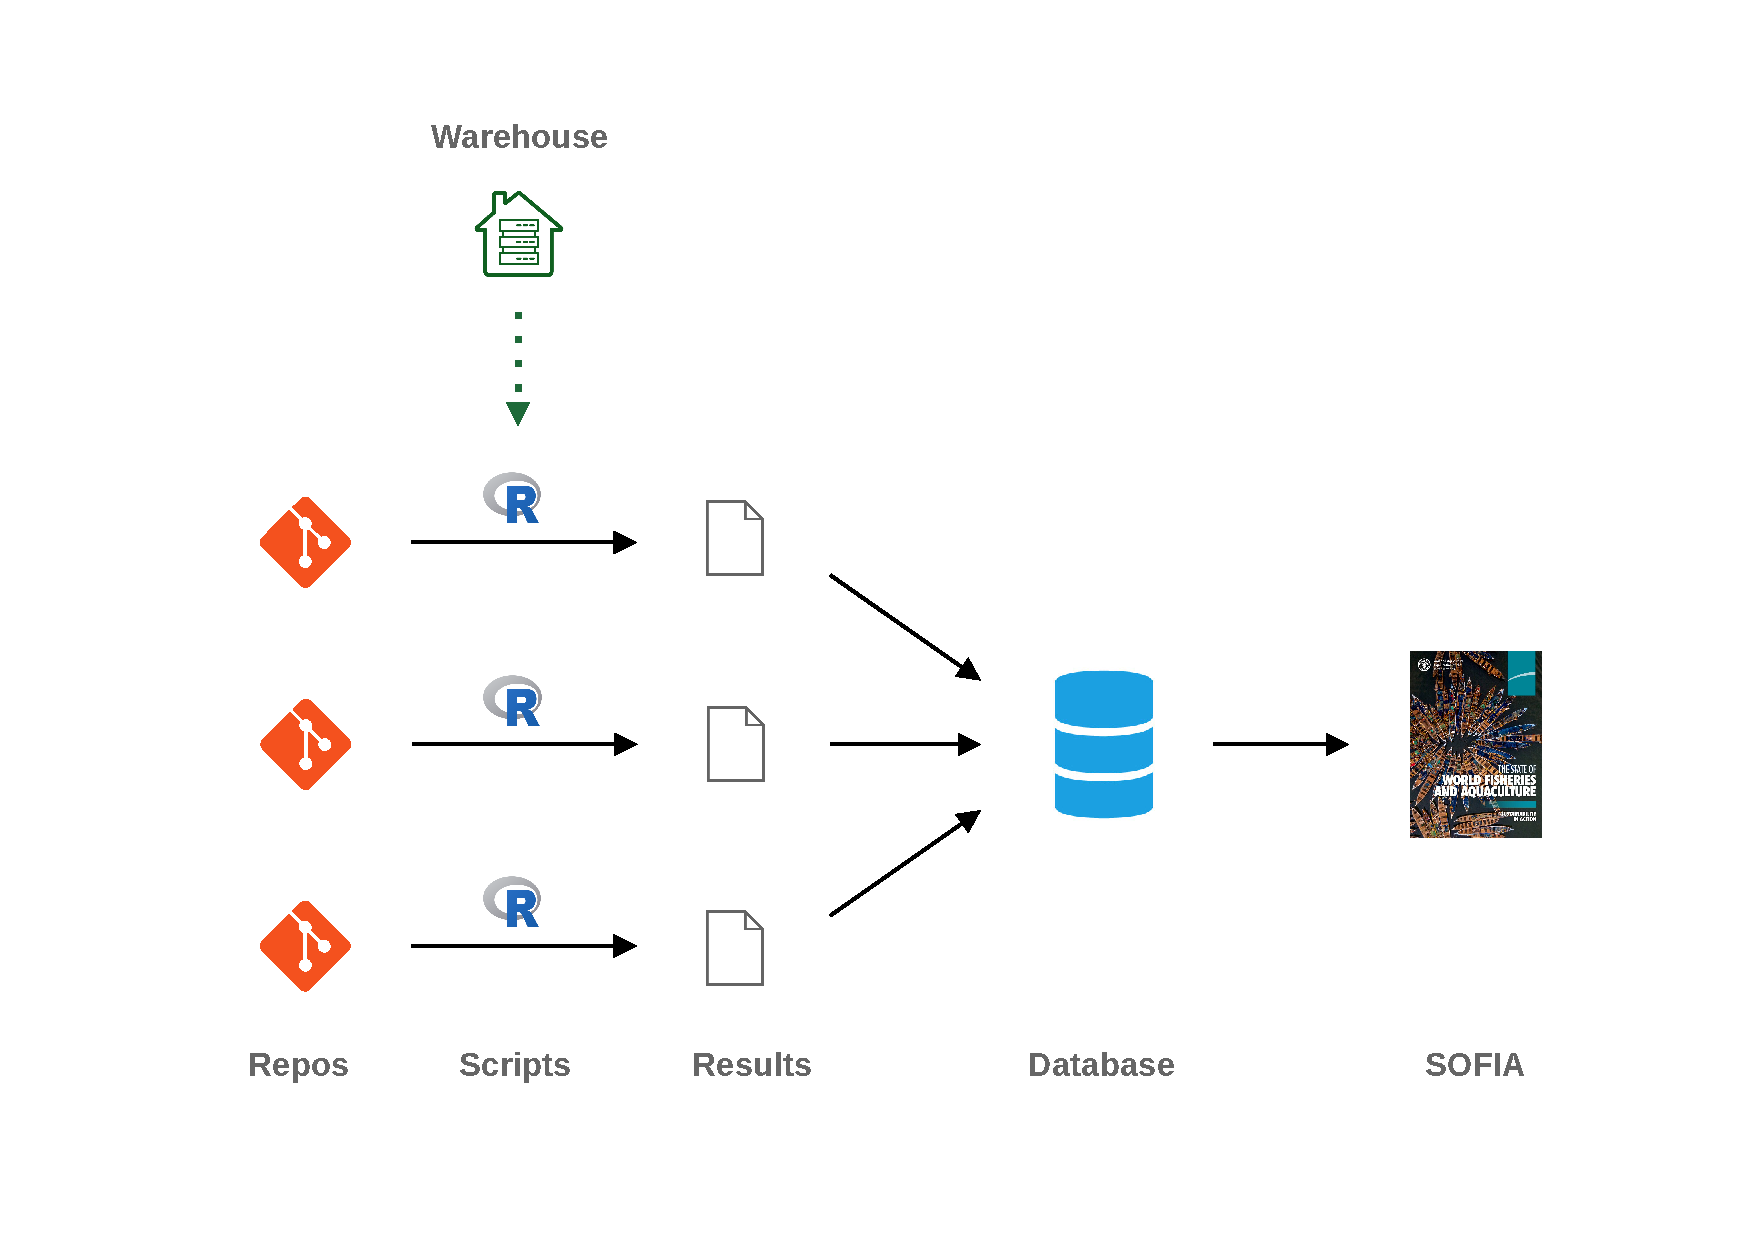
\includegraphics[width=0.8\textwidth]{tsaf_diagram}
    \vspace{2ex}
    \caption{TSAF diagram, showing the flow of information from individual
      repositories (analyses of stocks and areas) to the final SOFIA report.}
    \label{fig:tsaf-diagram}
  \end{center}
\end{figure}

The scripts use a dedicated R package called {\sf TSAF}. The next sections
describe each component of the TSAF design in some detail: repositories, input
data warehouse, R package, and the database.

\subsection{TSAF repositories}

\subsubsection{Repository features}

Each TSAF repository is a unit of analysis, corresponding to a specific area and
stocks. A GitHub repository, sometimes abbreviated as `repo', is an online
directory that is especially convenient for organizing text files, such as
scripts and data files. GitHub repository features relevant for TSAF include:

\begin{itemize}
  \item Ability to make scripts available online, for browsing and downloading,
  along with the input data required for the scripts to run.
  \item Automatic backup of all files with the ability to return to previous
  saved states.
  \item Tracked changes showing who changed what and when, supporting online
  teamwork.
  \item Ability to tag specific saved states of the analysis and give them
  descriptive names, such as `starting point`, `2021 data` or `results imported
  to database`.
  \item Ability to upload large attachments (\gt 100 MB) to accompany tagged
  states.
  \item Online facilities to compare text files and view changes, line by line.
\end{itemize}

\subsubsection{R scripts}

The analysis inside each repository consists of a set of R scripts that are
organized in TAF format (Magnusson and Millar 2021). This means there are four
standard scripts
(Table~\ref{tab:taf-scripts}) that conduct and document the analysis:\\[-1ex]

\begin{table}[htb]\small
  \caption{Standard TAF scripts for a given analysis.}
  \centering
  \begin{tabular}{ll}
    \hline
    Script          & Purpose\I{2.4ex}                                 \\
    \hline
    \verb|data.R|   & Preprocess data, write TAF data tables\I{2.6ex}  \\[0.6ex]
    \verb|model.R|  & Run analysis, write model results                \\[0.6ex]
    \verb|output.R| & Extract
                      results of interest, write TAF output tables     \\[0.6ex]
    \verb|report.R| & Prepare plots and formatted tables               \\[0.4ex]
    \hline
  \end{tabular}
  \label{tab:taf-scripts}
  \vspace{1.5ex}
\end{table}

The TAF scripts are run sequentially, each reading files that were created in a
previous step. The first script, \verb|data.R|, reads data files that were
declared and documented in a \verb|DATA.bib| text file. A similar
\verb|SOFTWARE.bib| file can be used to declare specific versions of software
used in the analysis, to strengthen reproducibility.

\begin{figure}[htb]
  \begin{center}
    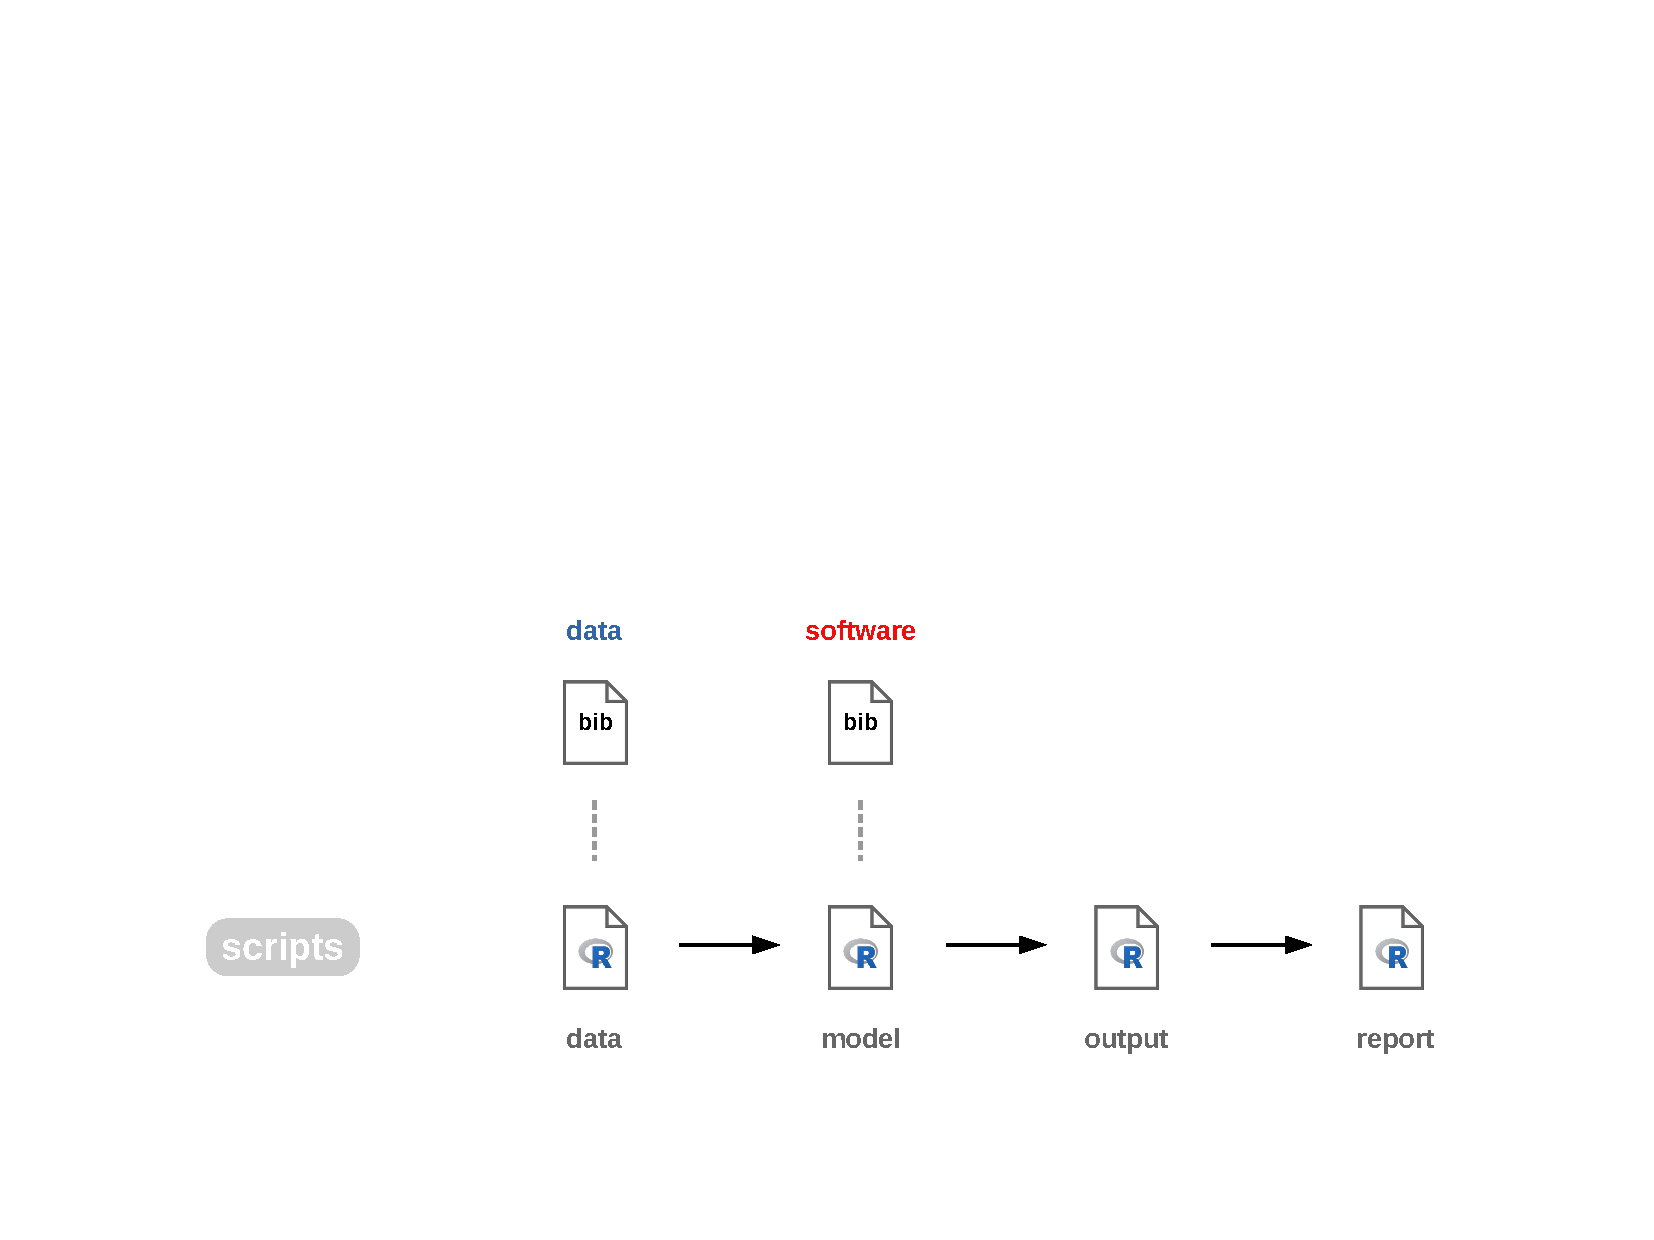
\includegraphics[width=0.8\textwidth]{taf_diagram}
    \vspace{2ex}
    \caption{TAF scripted workflow. Each TSAF repository/analysis contains four
      standard R~scripts that are run sequentially. The initial data and
      software are declared in so-called bib files.}
    \label{fig:taf-diagram}
  \end{center}
\end{figure}

\newpage

The R scripts conducting TSAF analyses rely especially on three R
packages:\\[-2ex]

\begin{itemize}
  \item {\sf TSAF} -- a new dedicated package to support TSAF\\
  (Sharma and Magnusson 2021)
  \item {\sf TAF} -- utilities to manage scripts, data files, metadata, and R
  data objects\\
  (Magnusson and Millar 2021)
  \item {\sf sraplus} -- biomass dynamics model with Bayesian priors\\
  (Ovando 2019)
\end{itemize}

\subsubsection{Repository names and directory structure}

GitHub repositories are given descriptive names, such as

\qquad\blue{\url{https://github.com/sofia-tsaf/2021Area37Coastal}}

for the analysis conducted in 2021 of coastal stocks in Area 37.

On a personal laptop or a high-performance cluster, the TSAF repositories are
organized in a hierarchical directory structure (Figure \ref{fig:tsaf-dirs}),
similar to the repository name as year/area/stock group.\\

\begin{figure}[htb]
  \begin{center}
    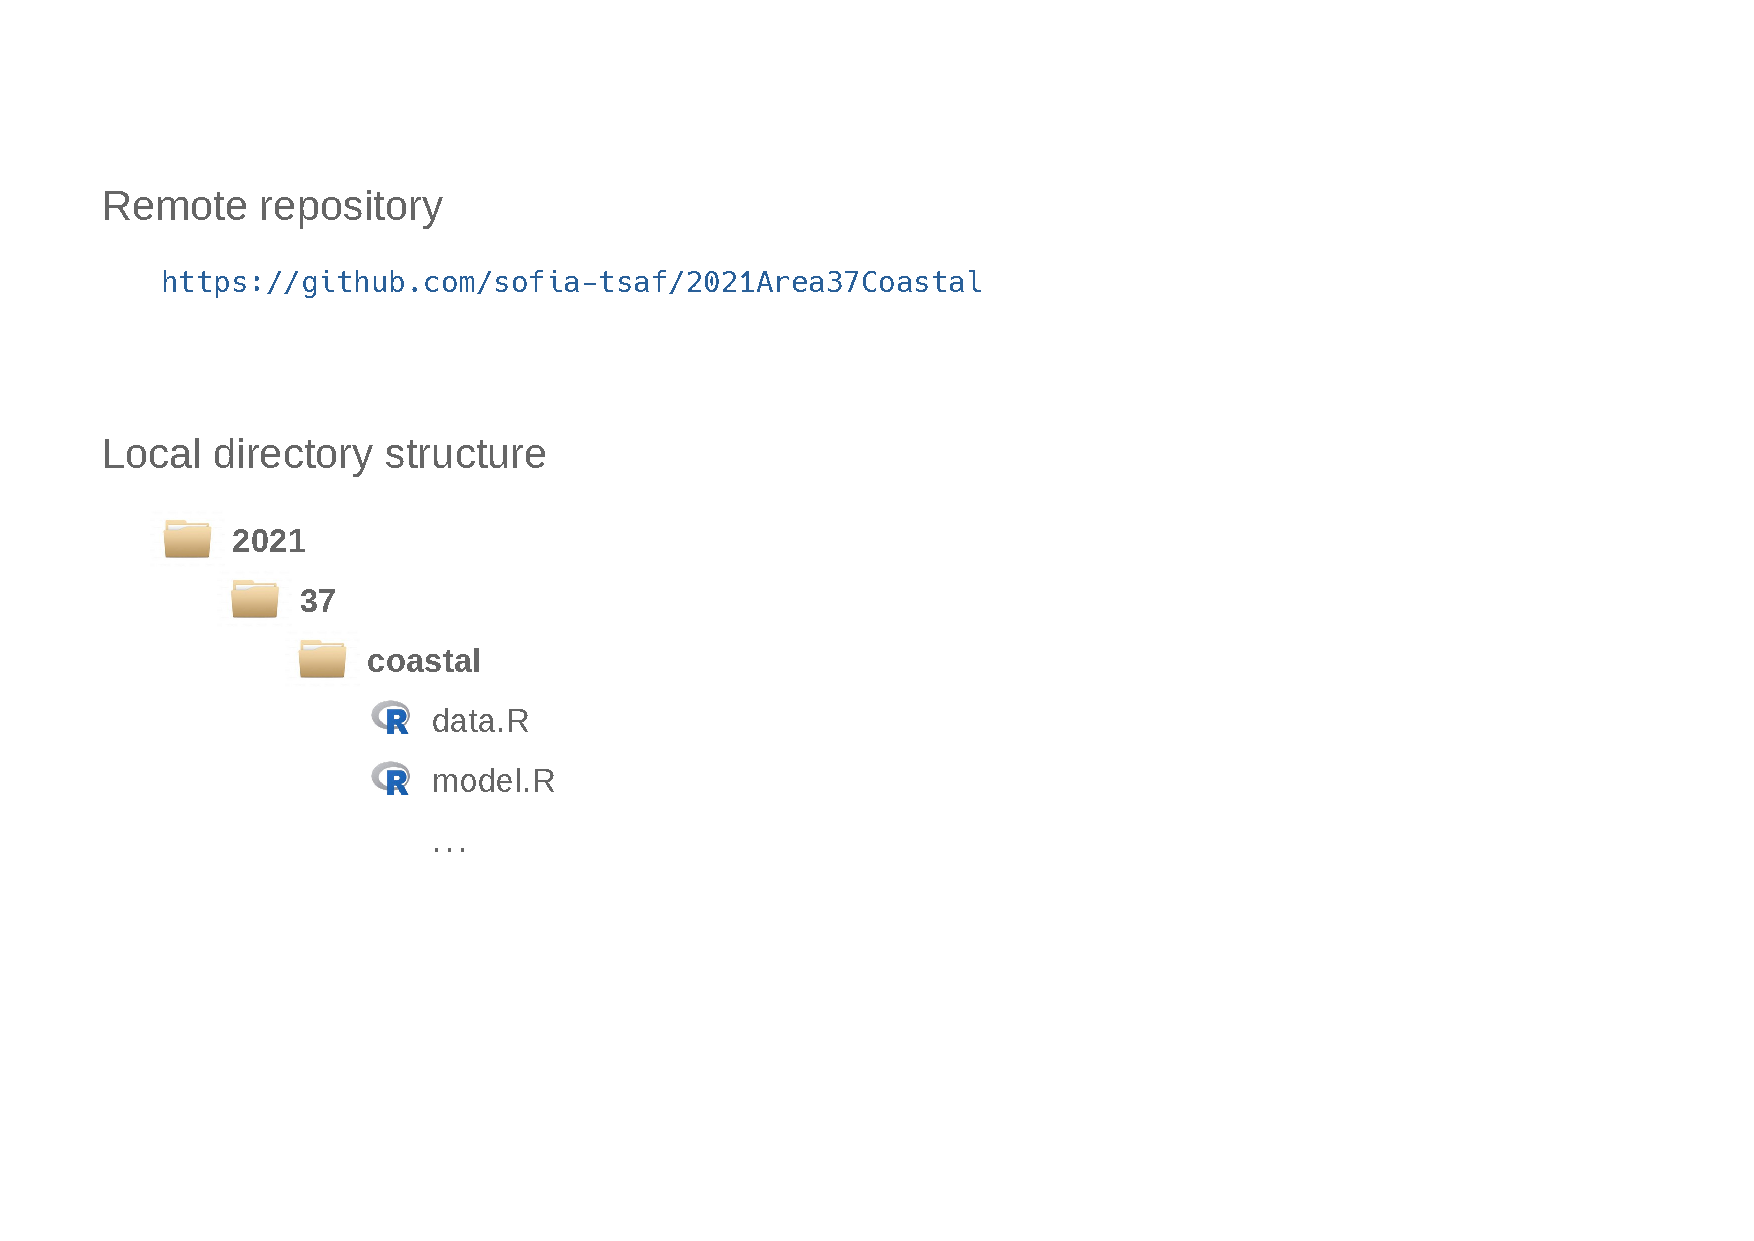
\includegraphics[width=0.6\textwidth]{tsaf_dirs}
    \vspace{1ex}
    \caption{TSAF local directory structure, showing the similarity between the
      remote repository name and the local directory names.}
    \label{fig:tsaf-dirs}
  \end{center}
\end{figure}

\vspace{1ex}

This hierarchical directory structure is practical to navigate and run the
analyses, access results, and run top-level summary calculations across a large
number of analyses.

\subsection{Input data warehouse}

The input data warehouse contains fisheries data for all areas and stocks. For
TSAF analyses of Tier 2 stocks, the focus is on catch and effort data, which are
organized in two GitHub repositories:

\qquad\blue{\url{https://github.com/sofia-tsaf/catches}}

\qquad\blue{\url{https://github.com/sofia-tsaf/effort}}

Individual TSAF analyses start by reading catch and effort data from the data
warehouse. In this way, the input data for all analyses are stored in one
central place, where they can be updated, documented, and quality checked.

\subsection{R package}

The {\sf TSAF} package (Sharma and Magnusson 2021) contains utilities that are
commonly used in TSAF analyses. It is developed in a dedicated GitHub
repository:

\qquad\blue{\url{https://github.com/sofia-tsaf/TSAF}}

The {\sf TSAF} package provides a single place to modify a large number of TSAF
analyses. Incremental improvements become more manageable, e.g., changing the
format of a specific plot, without having to edit each and every TSAF analysis.
It also makes the R scripts for each analysis shorter and thus easier to read,
write, and maintain.

\subsection{Database}

The TSAF database will contain the results from all the individual TSAF
analyses. The primary focus of the database is on stock status, both in
numerical terms and in categorical terms: underfished, fully fished, and
overfished.

The database is the central node and key component of the TSAF design. The only
way to enter data into the database is via TSAF analyses, as indicated in the
TSAF diagram (Figure \ref{fig:tsaf-diagram}), and when TSAF analyses of a
specific areas and stocks are updated, the database is automatically updated.
Furthermore, the top-level analysis for the final SOFIA report, aggregating a
large number of TSAF analyses, should be based on queries to the database.

The above design guarantees the traceability of SOFIA results, all the way from
the individual datasets and analyses to the final published report.

The database is also a convenient stage in the pipeline to apply quality
control. Examples of quality checks could include referential integrity of
species and stock names, summary statistics at different levels of aggregation,
counting stocks in each area, plotting the distribution of numerical stock
status, etc. This will ensure that all stocks are accounted for, and reveal any
inconsistencies or issues that should be checked in the underlying analyses.

% ______________________________________________________________________________

\section{Development status and next steps}

\subsection{TSAF repositories}

\subsubsection{Current status}

As of end of December 2021, the GitHub site
\blue{\url{https://github.com/sofia-tsaf}} contains 12 TSAF repositories:

\begin{verbatim}
  area31
  area37
  2021Area37Clams
  2021Area37Coastal
  2021Area37Cods
  2021Area37Demersal
  2021Area37Flounder
  2021Area37Herring
  2021Area37Other
  2021Area37Shads
  2021Area37Shrimps
  2021Area37Squid
\end{verbatim}

The status of all of these analyses is exploratory for development purposes, as
opposed to production analyses for a final SOFIA report.

The initial step in TSAF development focused on \verb|area31| and \verb|area37|,
which are aggregated analyses where all stocks within an area share the same
annual effort series, as well as priors on historical and current stock status.
These prototype analyses proved valuable to test and extend the early TSAF
design.

In the next step of TSAF development, the analysis of Area 37 was divided into
stock groups (clams, costal, cods, etc.), allowing stock groups to have
different effort series and priors.

The current TSAF development focuses on allowing full detailed control in the
analysis, where each species within a stock group can have different effort
series and priors. To manage these model settings, new R functions were
developed called \verb|addEffort| and \verb|addDriors|. Encapsulating these
actions in functions, that are defined and maintained outside the main scripts,
also comes with the side benefit of shortening and simplifying the scripts.
These latest developments have used the \verb|2021Area37Coastal| analysis as a
test case.

\subsubsection{Next steps}
\label{subsubsec:repos-next-steps}

\textbf{Read from input data warehouse}

Currently, the TSAF analyses read the initial catch and effort data from a local
data directory, specific to each analysis. This means that data are repeated
between analyses, especially the effort data. Furthermore, to update catch and
effort data, one would have to modify a large number of TSAF repositories. The
input data warehouse offers a more efficient, traceable, and quality-controlled
workflow.\\[-2ex]

\textbf{Categorical status by stock and year}

Currently, the TSAF analyses produce an output file called
\verb|stock_timeseries.csv| with numerical $B/B_\mathrm{MSY}$ and
$F/F_\mathrm{MSY}$ by stock and year. For the subsequent analysis, it would be
beneficial if the categorical stock status (underfished, fully fished,
overfished) by year is also included in this file. This improvement will require
modifications to the \verb|output.R| script of all TSAF analyses.\\[-2ex]

\textbf{Standardize and shorten scripts}

The main difference between the TSAF analyses that have been developed so far is
the underlying catch and effort data. Other model input, such as priors, is also
specified in dedicated input files. The benefit of this design is that the
analytical scripts (\verb|data.R|, \verb|model.R|, \verb|output.R|, and
\verb|report.R|) are almost identical between different TSAF repositories.

As the number of TSAF repositories grows, it becomes more cumbersome to make the
same change across all analyses. A simple change, such as a minor improvement in
the format of a specific plot, may involve modifying one line in a particular
script across all TSAF repositories.

The recent creation of the {\sf TSAF} package was an important step to provide a
single place to organize TSAF code that is shared between analyses. Moving
blocks of code from the R scripts into the {\sf TSAF} package, as encapsulated
and documented functions, will be beneficial for the development and maintenance
of TSAF analyses.

A thorough research and review of the TSAF analyses is required to identify
blocks of code that can be moved to shared functions. The design and development
of these functions and maintenance of the {\sf TSAF} package will be a good
investment to efficiently handle a large number of TSAF analyses.\\[-2ex]

\textbf{Reference analysis}

As the development of TSAF analyses continues, it might be practical to have one
reference analysis that demonstrates the latest features and recommended as a
template for creating a new TSAF analysis. Currently, the
\verb|2021Area37Coastal| analysis serves as the test case for new features and
improvements, but a dedicated reference analysis would be beneficial.\\[-2ex]

\textbf{Managing output files}

A significant challenge in TSAF is that each analysis takes considerable time to
run (\gt 1 hr) and produces large output files (\gt 100 MB). Every time a small
update is made to the scripts or underlying data, a new run is required and the
output files are likely to change. TSAF development so far has explored two
approaches to store the output files.

Approach 1. Initial development (e.g., \verb|area37|) kept the output files
outside of the repository. Instead of uploading the output files along with the
R scripts, output files were uploaded as GitHub `release assets'. The advantage
of this approach is that the repository remains very light and easy to work
with, and takes much less space on the hard drive of a personal laptop.

Approach 2. Later development (e.g., \verb|2021Area37Coastal|) has the output
files stored inside the repository. The advantage of this approach is that it
reduces the need to manage tags and GitHub releases, and makes it slightly less
likely to have mismatching R scripts and output files.

Unfortunately, neither of the above approaches can guarantee a correct match
between the R scripts and the output files. In other words, when a change is
made to an R script and uploaded to the repository, it's easy to forget or omit
running the entire analysis and uploading new output files.

A 3rd approach worth exploring would be not to upload output files to the GitHub
repository at all. Instead, the database server would run all analyses locally.
Specifically, a GitHub webhook could be developed, so that whenever a change is
uploaded to the GitHub repository, the database server pulls the changes, runs
the analysis and imports the results into the database. This would guarantee a
strong linkage between the TSAF repositories and the database.\\[-2ex]

\textbf{Other improvements in TSAF repositories}

In upcoming meetings, the TSAF development team will continue to use the TSAF
project board (Section \ref{subsec:project-board}) to discuss, prioritize, and
track the above and additional developments related to TSAF repositories.

\subsection{Input data warehouse}

\subsubsection{Current status}

The \blue{\url{https://github.com/sofia-tsaf/catches}} repository currently
contains the following files with catch data:

\begin{verbatim}
  cap_2021-10-17_193245.csv
  cap_all_area37_2021-10-12_64848.csv
  cap_flagged_2021-10-12_70055.csv
  cap_flagged_area37_2021-10-12_63449.csv
\end{verbatim}

The \blue{\url{https://github.com/sofia-tsaf/effort}} repository has been
created but is still empty.

\subsubsection{Next steps}

The data in the \verb|catches| repository data are ready for exploratory use,
testing the ability of R scripts to read catch data from the central warehouse
instead of a local data directory.

Data can be added to the \verb|effort| repository in CSV format. Alternative
structures of the data will be evaluated, before deciding how to organize the
effort data from different areas and stocks.

For TSAF analyses of Tier 1 and 3, the data warehouse can incorporate the
underlying numerical and categorical data from official stock assessments and
expert elicitation. This could further increase the clarity and traceability of
the overall SOFIA analysis of stock status.

\subsection{R package}

\subsubsection{Current status}

Version 1.0.0 of the {\sf TSAF} package was released on 10 Dec 2021. The package
help page that comes with {\sf TSAF} lists the following functions, categorized
by functionality.\\[-2ex]

{\it Prepare data:}

\begin{tabular}{ll}
  {\tt addDriors} & add `driors' (data and priors) column to stocks object\\
  {\tt addEffort} & add effort column to catch data\\[1.5ex]
\end{tabular}

{\it Calculate:}

\begin{tabular}{ll}
  {\tt calcCat} & stock status categories\\[1.5ex]
\end{tabular}

{\it Plot:}

\begin{tabular}{ll}
  {\tt plotCat} & summary of stock status categories\\[1.5ex]
\end{tabular}

The current status of the package is stable and fully documented, passing a
strict \verb|R CMD --as-cran| quality check. It will not be submitted to be
published on CRAN, however, since it requires the {\sf sraplus} package that
does not fulfill the strict criteria of CRAN packages.

\subsubsection{Next steps}

The development goal to `Standardize and shorten scripts' (Section
\ref{subsubsec:repos-next-steps}) involves extending the {\sf TSAF} package.
Specific ideas for additional functions have not yet been formulated.

\subsection{Database}

\subsubsection{Current status}

The database of TSAF results is implemented in MySQL. Its development is
organized in a GitHub repository:

\qquad\blue{\url{https://github.com/sofia-tsaf/database}}

Database import and export is managed using Bash shell scripts, which are found
in the GitHub repository.

\subsubsection{Next steps}

\textbf{Strong link between repositories and database}

The link between TSAF repositories and the database of results (Figure
\ref{fig:tsaf-diagram}) is essential for traceability and the fundamental
purpose of TSAF. The very basis of the TSAF design is that the results found in
the database should match exactly the results produced by the TSAF repositories.

One database script under development loops through the list of repositories and
pulls down the \verb|current_status.csv| file to ingest to the database.

The design and development of this linkage is still ongoing. It might be
beneficial to maintain a list of TSAF repositories whose results should be
imported into the database. Several repositories on
\blue{\url{https://github.com/sofia-tsaf}} are not TSAF analyses producing
results for the database, e.g., software development repositories, input data
warehouse repositories, and exploratory or reference analyses. The database
should import results from all relevant TSAF repositories, while omitting other
repositories.\\[-2ex]

\textbf{Database server managing TSAF output files}

One design possibility is to have a dedicated TSAF database server as the main
platform to run TSAF analyses and manage output files, in addition to importing
the results into the database.

The development goal `Managing output files' (Section
\ref{subsubsec:repos-next-steps}) elaborates on this possible approach, which
could involve a GitHub webhook to establish a reliable pipeline of information
from TSAF repositories to the database.

\newpage

\section{Acknowledgements}

Working with Rishi Sharma and Nicole Tursich on this project is a privilege and
joy. Our domains of expertise complement each other, and we share a common
vision and enthusiasm to enhance the FAO infrastructure and analytical workflows
for estimating the state of the world's fisheries. I would like to acknowledge
Colin Millar for our collaboration in creating TAF (Magnusson and Millar 2021),
which has served as an inspiration and basis for the TSAF design. Last but not
least, I~am grateful to Pedro Barros and colleagues at FAO for their guidance
and vote of confidence for this technical development project.\\[-1ex]

\section{References}

\small\sloppy\setlength\hyphenpenalty{1000}\selectfont
\begin{description}\setlength\itemsep{0.5ex}\vspace{0.5ex}

  \item FAO (Food and Agriculture Organization of the United Nations). 2020. The
  State of World Fisheries and Aquaculture 2020: Sustainability in action. Rome.
  206 pp.\\
  \blue{\footnotesize\url{https://doi.org/10.4060/ca9229en}}

  \item ICES (International Council for the Exploration of the Sea). 2021.
  Transparent Assessment Framework.\\
  \blue{\footnotesize\url{https://taf.ices.dk}}

  \item Magnusson, A. and C. Millar. 2021. TAF: Functions to Support the ICES
  Transparent Assessment Framework. R package version 4.0.0.\\
  \blue{\footnotesize\url{https://cran.r-project.org/package=TAF}}

  \item Ovando, D. 2019. sraplus: Run sraplus Assessments. R package version
  3.7.3.\\
  \blue{\footnotesize\url{https://github.com/DanOvando/sraplus}}

  \item Sharma, R. and A. Magnusson. 2021. TSAF: Tools to Work with SOFIA-TSAF
  Analyses. R package version 1.0.0.\\
  \blue{\footnotesize\url{https://github.com/sofia-tsaf/TSAF}}

\end{description}

\normalsize

\newpage

\appendix

\section{Arni's contributions in 2021}

\textbf{TSAF design}

The work on this project is divided been design and development. The design part
takes place largely during online technical meetings of the TSAF development
team, and is the product of dynamic teamwork and discussions. As the TSAF design
borrows both ideas and technical components from TAF (Magnusson and Millar
2021), Arni has served in a lead role in the design of many aspects of TSAF,
especially the structure of TSAF repositories, input data warehouse, and the
R~package.\\[-2ex]

\textbf{TSAF repository development}

On the development front, Arni started by creating the \verb|area37| repository,
demonstrating how a TSAF analysis can be efficiently divided into four scripts
(\verb|data.R|, \verb|model.R|, \verb|output.R|, and \verb|report.R|) and taking
advantage of the existing TAF package to support reproducibility. He then made
incremental improvements to the \verb|area37| analysis, giving objects and files
short and generic names that can be used consistently between different SOFIA
analyses. The \verb|area37| repository served as a template for all later TSAF
repositories.\\[-2ex]

\textbf{Teaching and documenting}

Since the other development team members were rather new to using GitHub
repositories and TAF workflows, Arni has dedicated project time to teaching and
documenting how those technologies are used in TSAF. He also analyzed the extent
of package dependencies of the {\sf sraplus} package, which is especially
relevant for the reproducibility aspect of TSAF analyses.\\[-2ex]

\textbf{Stock-specific analysis}

Later development focus of Arni's work was the generalization of TSAF analyses,
to allow effort data and priors to be either stock-specific or shared across
stocks. This improvement was first implemented as a general structure for the
input data files and a revised block of code in the \verb|data.R| script of
analysis \verb|2021Area37Coastal|. To select which analytical option to use, a
flag \verb|stocks.combined| in the data script is set to \verb|TRUE| or
\verb|FALSE|, with corresponding if-constructs added to the code. These
if-constructs were later replaced with a cleaner solution, as encapsulated
functions in a new dedicated {\sf TSAF} package.\\[-2ex]

\textbf{R package}

The new functionality of stock-specific analysis led Arni to develop a new R
package called {\sf TSAF} that is now operational. Acting as a single place of
analytical methods used in all TSAF analyses, greatly improving the ability
to manage and maintain the large number of TSAF analyses behind SOFIA.\\[-2ex]

\newpage

\textbf{Contributions to project management}

Arni proposed and created the project board used to track TSAF development
progress, along with a discussion board, milestones, and issue tracker. Finally,
he wrote the current report, which consolidates the progress made so far,
conveys a design manifesto, documents existing features, and serves as a
foundation for the next steps and team discussions on TSAF development.\\[-2ex]

\textbf{Links to deliverables}

\begin{itemize}
  \item[-]\blue{\href{https://github.com/sofia-tsaf/area37}{{\sf area37}}}
  analysis\\[-3ex]
  \item[-]\blue{
    \href{https://github.com/sofia-tsaf/doc/blob/main/sraplus_dependencies.md}
    {{\sf sraplus}}} list of dependencies\\[-3ex]
  \item[-]\blue{\href{https://github.com/sofia-tsaf/project/projects/1}
    {\sf Project board}}
  \item[-]\blue{\href{https://github.com/sofia-tsaf/2021Area37Coastal}
    {{\sf 2021Area37Coastal}}} analysis\\[-3ex]
  \item[-]\blue{\href{https://github.com/sofia-tsaf/TSAF}{{\sf TSAF}}}
  package\\[-3ex]
  \item[-]\blue{\href{https://arni-magnusson.github.io/pdf/2021-tsaf.pdf}
    {{\sf This}}} current report
\end{itemize}

\end{document}
